\documentclass[a4paper]{report}

\usepackage{graphicx}

\newcounter{definitionNumber}
\renewcommand*\thedefinitionNumber{\thechapter.\arabic{definitionNumber}}

\newcommand{\definition}{ 
    \refstepcounter{definitionNumber}
    Definition \arabic{chapter}.\arabic{definitionNumber}.
}

\newcounter{lemmaNumber}
\renewcommand*\thelemmaNumber{\thechapter.\arabic{lemmaNumber}}

\newcommand{\lemma}{
    \refstepcounter{lemmaNumber}
    Lemma \arabic{chapter}.\arabic{lemmaNumber}.
}


\begin{document}

\chapter{Equivalence and Machine Minimization}
\section{Introduction}

In the preceding chapters it was emphasized that the state of a finite-state machine need not be observable or even physical quantitites, and that their only function is to assist in the formulation of the input-output relationships of the machine. Consequently, any state set which fulfills this function is a satisfactory set, regardless of whether the state convey any intuitive meaning or not. This freedom inherent in the choice of a state set is quite advantageous, since it permits the replacement of one set with another set which may be considered more convenient for various purposes. More specifically, it permits one to carry out operations aiming at producing a state set which is ``optimal'' or ``minimal'' in one sense or another. In all these considerations the concept of ``equivalence'' plays a major role. As will become apparent in this and later chapters, this concept not only paves the way for more precise and more concise formulation of finite-state machines, but sheds new light on the entire problem of machine analysis (as well as synthesis).

\section{State Equivalence}

In what follows, the notation $ M |\sigma $ will be used as an abbreviation for the phrase ``machine M in state $\sigma$''.

\definition \label{labelEquivalence}  State $ \sigma_i $ of machine $M_1$ and state $\sigma_j$ of machine $M_2$ are said to be \emph{equivalent}, if $M_1|\sigma_i$ and $M_2|\sigma_j$, when excited by any input sequence, yield identical output sequences. If $\sigma_i$ and $\sigma_j$ are not equivalent, they are said to be \emph{distinguishable}. $M_1$ and $M_2$ may refer to the same machine.

    Thus, $\sigma_i$ and $\sigma_j$ are equivalent if and only if there is no way of distinguishing, by observing the external terminals, between machine $M_1$ at the initial state $\sigma_i$ and Machine $M_2$ at the initial state $\sigma_j$. $\sigma_i$ and $\sigma_j$ are distinguishable if and only if there is at least one input sequence which, when applied to both $M_1|\sigma_i$ and $M_2|\sigma_j$, yields different output sequences.

    Equivalence between $\sigma_i$ and $\sigma_j$ is indicated by $\sigma_i = \sigma_j$, and distinguishability between $\sigma_i$ and $\sigma_j$ is indicated by  $\sigma_i \neq \sigma_j$. From definition \ref{labelEquivalence} it can be readily verified that state equivalence obeys the reflexive law ( $\sigma_i = \sigma_j$ ), the symmetric law ( if $\sigma_i = \sigma_j$, then $\sigma_j = \sigma_i$), and the transitive law  ( if $\sigma_i = \sigma_j$ and  $\sigma_j = \sigma_k$, then $\sigma_i = \sigma_k$). Consequently, state equivalence can be treated as an ordinary equivalence relation and applied directly to sets of states of any size. State distinguishability, on the other hand, does not obey the reflexive and transitive laws and, hence, can be applied only to pairs of states.

    In some cases equivalence or distinguishability of a pair of states belonging to the same machine can be estabilished by insoection of the transition table of this machine. Some of these cases are described by means of the following three lemmas. 

    %TODO: introduzir a subtable z_v

    \lemma \label{labelSimplyDistinct} Let $\sigma_i$ and $\sigma_j$ be states of machine M. If rows $\sigma_i$ and $\sigma_j$ in the $ z_v $ subtable of M are distinct, then $ \sigma_i \neq \sigma_j $.

    \emph{Proof}. There must be at least one input symbol which, when applied to $M|\sigma_i$ and $M|\sigma_j$, yields distinct output symbols. By definition \ref{labelEquivalence}, then $\sigma_i \neq \sigma_j$.


    \lemma \label{labelSimplyEquiv} Let $\sigma_i$ and $\sigma_j$ be states of machine M. If rows $\sigma_i$ and $\sigma_j$, spanning the entire transition table of M, are identical, then $\sigma_i = \sigma_j$.

    \emph{Proof}. When any input symbol is applied to $M_1|\sigma_i$ and $M_2|\sigma_j$, the output symbols and next states are identical in the two alternatives. Once $M_1|\sigma_i$ and $M_2|\sigma_j$ pass into the same state, their responses to all subsequent excitations must coincide. By definition \ref{labelEquivalence}, then, $\sigma_i = \sigma_j$.

    \lemma \label{labelSimplyModifiedEquiv} Let $\sigma_i$ and $\sigma_j$ be states of machine M. If rows $\sigma_i$ and $\sigma_j$, spanning the entire transition table of M, become identical when every $\sigma_i$ is replaced by $\sigma_j$ (or every $\sigma_j$ is replaced by $\sigma_i$), then $\sigma_i = \sigma_j$.

    \emph{Proof}. When any input symbol is applied to $M|\sigma_i$ and $M|\sigma_j$, the output symbols are identical in the two alternatives. $M|\sigma_i$ and $M|\sigma_j$ either pass into the same state or into states $\sigma_i$ and $\sigma_j$ (not necessarily respectively). If the next state is the same, their responses to all subsequent excitations must coincide. If the next states are $\sigma_i$ and $\sigma_j$, the original situation is restored and the above argument can be repeated to show that the next output symbols are identical in the two alternatives. By induction, then, the responses of $\sigma_i$ and $\sigma_j$ to any input sequence are identical, which implies that $\sigma_i = \sigma_j$.

    Pairs of rows which exhibit the property cited in Lemma \ref{labelSimplyDistinct} are said to be \emph{simply distinguishable}, and states in the stub of these rows are called simply distinguishable states. Pairs of rows which exhibit the property cited in Lemma \ref{labelSimplyEquiv} or Lemma \ref{labelSimplyModifiedEquiv} are said to be \emph{simply equivalent}, and the states in the stub of these rows are called simply equivalent states.
    We thus have:

    \theorem \label{labelSimplyTheorem} If $\sigma_i$ and $\sigma_j$ are simply distinguishable, then $\sigma_i \neq \sigma_j $. If $\sigma_i$ and $\sigma_j$ are simply equivalent, then $\sigma_i = \sigma_j $.

    % TODO: introduzir as definicoes de classe da Sec. 2.3
    It should be pointed out that the converse of Theorem \ref{labelSimplyTheorem} is not true: not every distinguishable pair of states is simply distinguishable, and not every equivalent pair of states is simply equivalent. Using the class definitions introduced in Sec. 2.3, it can be concluded that in a simply minimal machine all pairs of states are distinguishable and in a simply reducible machine at least one pair of states is equivalent.

    \begin{figure}[!t]
        \centering
        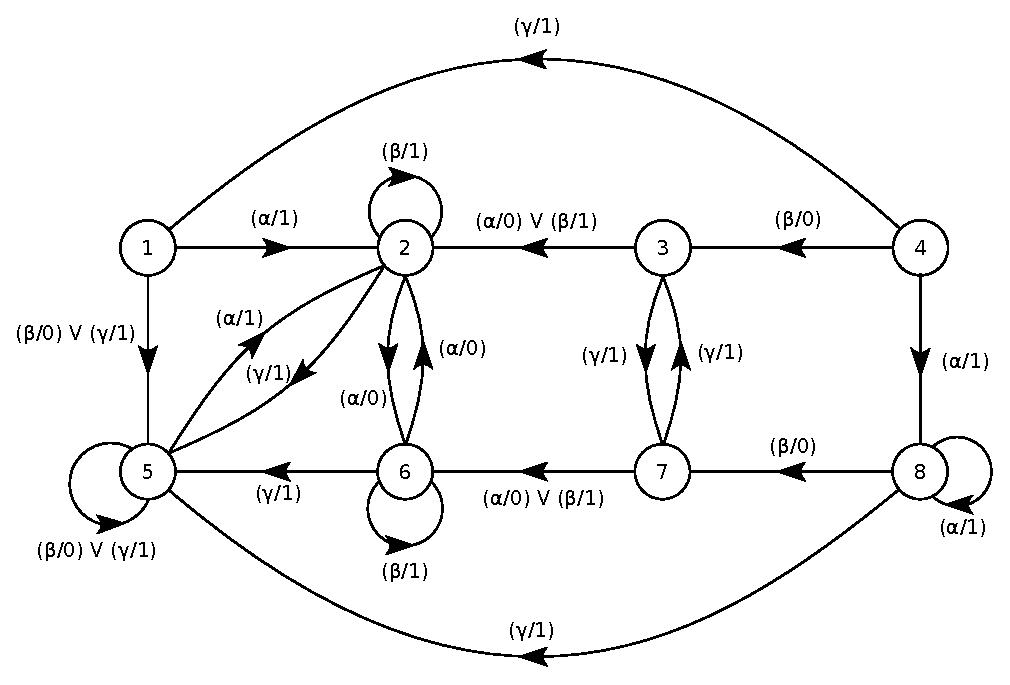
\includegraphics[width=256pt,clip]{images/eps/machineA6}
        \captionSampleMachine
        \label{fig:machineA6}
    \end{figure}


    %TODO: adicionar machine A6 e trocar referencias
    To illustrate Lemmas \ref{labelSimplyDistinct} to \ref{labelSimplyModifiedEquiv}, consider figure \ref{fig:machineA6}, specified by 

\end{document}
